\chapter{Functional Magnetic Resonance Imaging (fMRI)}
\label{ch:functional_mri}

% Chapter-opening illustrated modality infographic.
\begin{center}
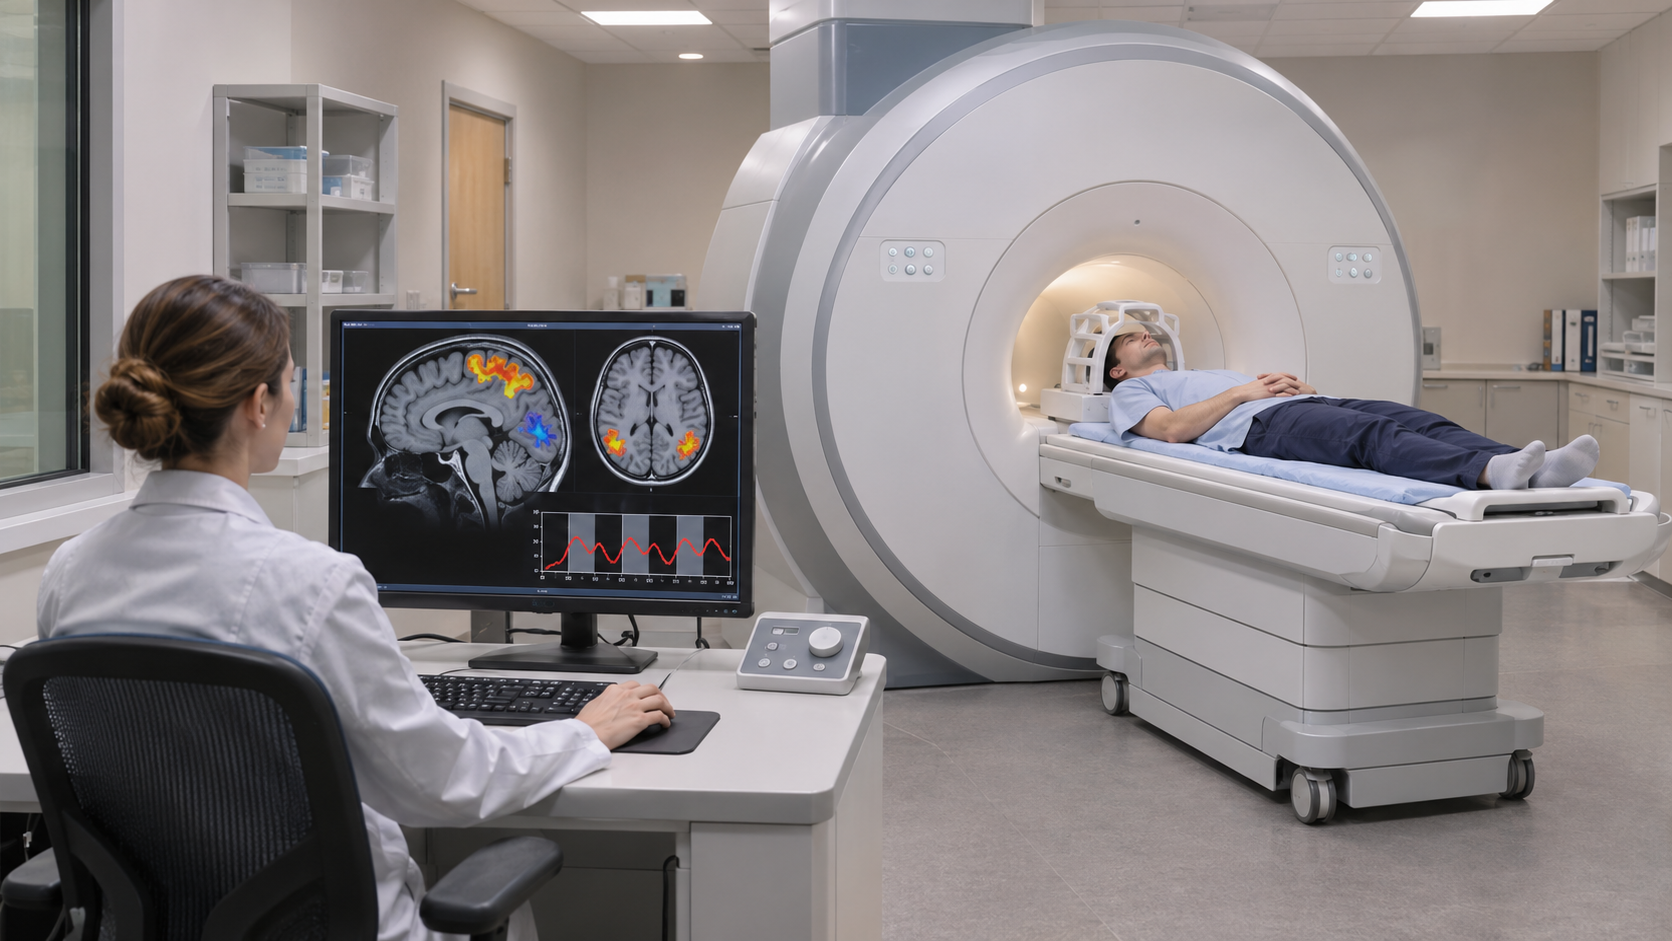
\includegraphics[width=\textwidth,keepaspectratio]{modalities/infographics/fmri_realistic.png}
\end{center}
\begin{center}\footnotesize BOLD fMRI maps task-related changes in blood oxygenation, an indirect hemodynamic signal rather than a direct recording of neuronal firing. AI-generated illustration; activation maps are not research data.\end{center}

\section{Overview}
Functional magnetic resonance imaging (fMRI) is a specialized MRI technique that measures changes in blood oxygenation and hemodynamics associated with neuronal activity. Most clinical and research applications use the blood oxygen level-dependent (BOLD) signal.

Unlike conventional MRI, which primarily examines anatomical and pathological abnormalities, fMRI investigates functional localization of brain regions, functional connectivity, reorganization of neural networks, abnormal activation patterns, cognitive, sensory and motor functions, and hemodynamic responses associated with neuronal activity.

fMRI is predominantly a research modality, with relatively limited routine clinical applications. Presurgical motor and language mapping are established clinical uses in selected cases. Many reported associations in the catalogues below are group-level research findings and are not validated as individual diagnostic tests.

 Individual findings have not been independently verified against published studies or clinical guidelines.

\section{Where fMRI is used}
The numbered entries summarize examples of conditions studied with fMRI and reported functional patterns. Findings are influenced by task design, patient performance, head motion, vascular physiology, acquisition parameters, and analysis methods.

\subsection{Brain tumors and presurgical planning}
\begin{enumerate}[leftmargin=*,itemsep=0.45em,topsep=0.4em]
\item \textbf{Astrocytoma.} Useful imaging findings include: Altered activation near tumor boundaries.
\item \textbf{Brain metastases.} Useful imaging findings include: Altered activation near metastatic lesions.
\item \textbf{Brainstem tumors.} Useful imaging findings include: Possible alterations in functional networks.
\item \textbf{Cavernous malformation.} Useful imaging findings include: Functional cortical activation adjacent to the lesion.
\item \textbf{Cerebral arteriovenous malformation.} Useful imaging findings include: Altered functional localization and neurovascular coupling.
\item \textbf{Glioblastoma.} Useful imaging findings include: Displacement or reorganization of functional cortical regions.
\item \textbf{Low-grade glioma.} Useful imaging findings include: Functional cortical reorganization.
\item \textbf{Meningioma.} Useful imaging findings include: Displacement of functional cortical regions.
\item \textbf{Oligodendroglioma.} Useful imaging findings include: Reorganization of functional cortical networks.
\end{enumerate}
The principal purpose in these cases is to identify functionally important brain regions before surgery, rather than to diagnose the tumor itself.

\subsection{Epilepsy}
\begin{enumerate}[leftmargin=*,itemsep=0.45em,topsep=0.4em]
\item \textbf{Childhood absence epilepsy.} Useful imaging findings include: Altered thalamocortical network activity.
\item \textbf{Drug-resistant epilepsy.} Useful imaging findings include: Functional reorganization of language and memory networks.
\item \textbf{Focal cortical dysplasia.} Useful imaging findings include: Abnormal regional functional activation.
\item \textbf{Focal epilepsy.} Useful imaging findings include: Altered regional functional connectivity.
\item \textbf{Frontal lobe epilepsy.} Useful imaging findings include: Abnormal frontal network activity.
\item \textbf{Generalized epilepsy.} Useful imaging findings include: Abnormal thalamocortical connectivity.
\item \textbf{Juvenile myoclonic epilepsy.} Useful imaging findings include: Altered motor and cognitive network connectivity.
\item \textbf{Lennox--Gastaut syndrome.} Useful imaging findings include: Altered widespread cortical and subcortical networks.
\item \textbf{Mesial temporal sclerosis.} Useful imaging findings include: Altered hippocampal activation and connectivity.
\item \textbf{Temporal lobe epilepsy.} Useful imaging findings include: Altered temporal lobe functional connectivity.
\end{enumerate}
Presurgical language lateralization is an established clinical application. Simultaneous EEG-fMRI for localization of epileptic activity remains more specialized.

\subsection{Cerebrovascular diseases}
\begin{enumerate}[leftmargin=*,itemsep=0.45em,topsep=0.4em]
\item \textbf{Carotid artery stenosis.} Useful imaging findings include: Altered cerebrovascular reactivity.
\item \textbf{Cerebral small vessel disease.} Useful imaging findings include: Reduced or altered functional connectivity.
\item \textbf{Chronic cerebral ischemia.} Useful imaging findings include: Abnormal hemodynamic responses.
\item \textbf{Hemorrhagic stroke.} Useful imaging findings include: Functional network disruption.
\item \textbf{Ischemic stroke.} Useful imaging findings include: Altered activation within affected functional networks.
\item \textbf{Moyamoya disease.} Useful imaging findings include: Impaired or delayed cerebrovascular reactivity.
\item \textbf{Post-stroke aphasia.} Useful imaging findings include: Reorganization of language networks.
\item \textbf{Post-stroke cognitive impairment.} Useful imaging findings include: Altered executive and attention networks.
\item \textbf{Post-stroke motor impairment.} Useful imaging findings include: Altered sensorimotor cortical activation.
\item \textbf{Vascular dementia.} Useful imaging findings include: Disrupted large-scale neural networks.
\end{enumerate}

\subsection{Neurodegenerative diseases}
\begin{enumerate}[leftmargin=*,itemsep=0.45em,topsep=0.4em]
\item \textbf{Alzheimer disease.} Useful imaging findings include: Altered default mode network connectivity.
\item \textbf{Amyotrophic lateral sclerosis.} Useful imaging findings include: Altered motor network connectivity.
\item \textbf{Dementia with Lewy bodies.} Useful imaging findings include: Altered visual and attention networks.
\item \textbf{Frontotemporal dementia.} Useful imaging findings include: Disrupted frontal and temporal networks.
\item \textbf{Huntington disease.} Useful imaging findings include: Altered corticostriatal functional connectivity.
\item \textbf{Mild cognitive impairment.} Useful imaging findings include: Altered hippocampal and cortical connectivity.
\item \textbf{Multiple system atrophy.} Useful imaging findings include: Altered cerebellar and motor connectivity.
\item \textbf{Parkinson disease.} Useful imaging findings include: Abnormal corticostriatal connectivity.
\item \textbf{Posterior cortical atrophy.} Useful imaging findings include: Altered posterior cortical networks.
\item \textbf{Primary progressive aphasia.} Useful imaging findings include: Disrupted language networks.
\item \textbf{Progressive supranuclear palsy.} Useful imaging findings include: Disrupted brainstem and frontal networks.
\item \textbf{Spinocerebellar ataxia.} Useful imaging findings include: Abnormal cerebellocortical connectivity.
\end{enumerate}

\subsection{Psychiatric disorders}
\begin{enumerate}[leftmargin=*,itemsep=0.45em,topsep=0.4em]
\item \textbf{Alcohol use disorder.} Useful imaging findings include: Altered reward and executive networks.
\item \textbf{Anorexia nervosa.} Useful imaging findings include: Altered reward and body perception networks.
\item \textbf{Binge-eating disorder.} Useful imaging findings include: Altered food-related reward responses.
\item \textbf{Bipolar disorder.} Useful imaging findings include: Abnormal emotional regulation networks.
\item \textbf{Borderline personality disorder.} Useful imaging findings include: Altered emotional regulation networks.
\item \textbf{Bulimia nervosa.} Useful imaging findings include: Altered reward and inhibitory control networks.
\item \textbf{Cocaine use disorder.} Useful imaging findings include: Altered reward and inhibitory control networks.
\item \textbf{Gambling disorder.} Useful imaging findings include: Altered reward-processing and decision-making networks.
\item \textbf{Generalized anxiety disorder.} Useful imaging findings include: Altered amygdala-prefrontal connectivity.
\item \textbf{Major depressive disorder.} Useful imaging findings include: Altered limbic and prefrontal connectivity.
\item \textbf{Nicotine dependence.} Useful imaging findings include: Altered cue-related reward network activation.
\item \textbf{Obsessive-compulsive disorder.} Useful imaging findings include: Altered corticostriatal-thalamocortical connectivity.
\item \textbf{Opioid use disorder.} Useful imaging findings include: Altered reward and motivational circuitry.
\item \textbf{Panic disorder.} Useful imaging findings include: Abnormal fear-processing network activity.
\item \textbf{Post-traumatic stress disorder.} Useful imaging findings include: Altered amygdala, hippocampal and prefrontal responses.
\item \textbf{Schizophrenia.} Useful imaging findings include: Disrupted large-scale functional connectivity.
\item \textbf{Social anxiety disorder.} Useful imaging findings include: Altered responses to socially threatening stimuli.
\item \textbf{Specific phobia.} Useful imaging findings include: Increased activation of fear-related networks during exposure.
\end{enumerate}
These disorders cannot currently be reliably diagnosed in an individual patient using fMRI alone. Most reported findings represent statistical differences between research populations.

\subsection{Neurodevelopmental disorders}
\begin{enumerate}[leftmargin=*,itemsep=0.45em,topsep=0.4em]
\item \textbf{Attention deficit hyperactivity disorder.} Useful imaging findings include: Altered attention and executive control networks.
\item \textbf{Autism spectrum disorder.} Useful imaging findings include: Altered social cognition and functional connectivity networks.
\item \textbf{Cerebral palsy.} Useful imaging findings include: Functional reorganization of motor networks.
\item \textbf{Developmental dyscalculia.} Useful imaging findings include: Altered numerical processing networks.
\item \textbf{Developmental dyslexia.} Useful imaging findings include: Altered activation of reading-related networks.
\item \textbf{Developmental language disorder.} Useful imaging findings include: Altered language network activation.
\item \textbf{Down syndrome.} Useful imaging findings include: Altered large-scale functional connectivity.
\item \textbf{Fragile X syndrome.} Useful imaging findings include: Abnormal cognitive and emotional processing networks.
\item \textbf{Rett syndrome.} Useful imaging findings include: Altered sensorimotor and cognitive networks.
\item \textbf{Tourette syndrome.} Useful imaging findings include: Altered corticostriatal motor circuitry.
\item \textbf{Williams syndrome.} Useful imaging findings include: Altered visuospatial and social processing networks.
\end{enumerate}

\subsection{Demyelinating and inflammatory neurological diseases}
\begin{enumerate}[leftmargin=*,itemsep=0.45em,topsep=0.4em]
\item \textbf{Anti-NMDA receptor encephalitis.} Useful imaging findings include: Altered hippocampal and large-scale connectivity.
\item \textbf{Autoimmune encephalitis.} Useful imaging findings include: Disrupted cognitive and limbic networks.
\item \textbf{Multiple sclerosis.} Useful imaging findings include: Altered functional connectivity and compensatory cortical activation.
\item \textbf{Neuromyelitis optica spectrum disorder.} Useful imaging findings include: Altered visual and sensorimotor networks.
\item \textbf{Neuropsychiatric systemic lupus erythematosus.} Useful imaging findings include: Altered cognitive and emotional networks.
\end{enumerate}

\subsection{Traumatic brain injuries and disorders of consciousness}
\begin{enumerate}[leftmargin=*,itemsep=0.45em,topsep=0.4em]
\item \textbf{Cognitive motor dissociation.} Useful imaging findings include: Task-related brain activation despite absent observable behavioral response.
\item \textbf{Diffuse axonal injury.} Useful imaging findings include: Reduced or altered functional network connectivity.
\item \textbf{Disorders of consciousness.} Useful imaging findings include: Altered default mode and frontoparietal networks.
\item \textbf{Hypoxic brain injury.} Useful imaging findings include: Disrupted cortical and subcortical connectivity.
\item \textbf{Mild traumatic brain injury.} Useful imaging findings include: Altered functional connectivity.
\item \textbf{Minimally conscious state.} Useful imaging findings include: Variable preservation of higher-order functional networks.
\item \textbf{Moderate traumatic brain injury.} Useful imaging findings include: Disruption of large-scale neural networks.
\item \textbf{Post-concussion syndrome.} Useful imaging findings include: Altered attention and executive networks.
\item \textbf{Severe traumatic brain injury.} Useful imaging findings include: Extensive functional network abnormalities.
\item \textbf{Unresponsive wakefulness syndrome.} Useful imaging findings include: Reduced connectivity in consciousness-related networks; occasional covert task responses.
\end{enumerate}
Assessment of covert consciousness is an important emerging clinical application of task-based fMRI.

\subsection{Chronic pain and headache disorders}
\begin{enumerate}[leftmargin=*,itemsep=0.45em,topsep=0.4em]
\item \textbf{Chronic lower back pain.} Useful imaging findings include: Altered pain and emotional processing networks.
\item \textbf{Chronic pelvic pain.} Useful imaging findings include: Altered central pain-processing connectivity.
\item \textbf{Cluster headache.} Useful imaging findings include: Altered hypothalamic network activity.
\item \textbf{Complex regional pain syndrome.} Useful imaging findings include: Altered sensorimotor and pain networks.
\item \textbf{Fibromyalgia.} Useful imaging findings include: Altered central pain-processing networks.
\item \textbf{Irritable bowel syndrome.} Useful imaging findings include: Altered brain-gut processing networks.
\item \textbf{Migraine.} Useful imaging findings include: Altered sensory and pain-processing networks.
\item \textbf{Migraine with aura.} Useful imaging findings include: Altered visual cortical activity and hemodynamic responses.
\item \textbf{Neuropathic pain.} Useful imaging findings include: Abnormal somatosensory and pain-related connectivity.
\item \textbf{Phantom limb pain.} Useful imaging findings include: Altered sensorimotor cortical organization.
\item \textbf{Temporomandibular disorders.} Useful imaging findings include: Altered central pain-processing networks.
\item \textbf{Trigeminal neuralgia.} Useful imaging findings include: Altered pain-processing network activity.
\end{enumerate}

\subsection{Sensory disorders}
\begin{enumerate}[leftmargin=*,itemsep=0.45em,topsep=0.4em]
\item \textbf{Acquired blindness.} Useful imaging findings include: Altered visual cortical connectivity.
\item \textbf{Amblyopia.} Useful imaging findings include: Reduced or altered visual cortical responses.
\item \textbf{Anosmia.} Useful imaging findings include: Reduced olfactory-related cortical activation.
\item \textbf{Congenital blindness.} Useful imaging findings include: Cross-modal reorganization of the visual cortex.
\item \textbf{Congenital deafness.} Useful imaging findings include: Cross-modal reorganization of auditory regions.
\item \textbf{Glaucoma.} Useful imaging findings include: Altered visual pathway functional connectivity.
\item \textbf{Optic neuritis.} Useful imaging findings include: Altered visual cortical activation.
\item \textbf{Sensorineural hearing loss.} Useful imaging findings include: Altered auditory cortical activity.
\item \textbf{Tinnitus.} Useful imaging findings include: Altered auditory and limbic network activity.
\item \textbf{Vestibular disorders.} Useful imaging findings include: Altered vestibular processing networks.
\end{enumerate}

\subsection{Sleep disorders}
\begin{enumerate}[leftmargin=*,itemsep=0.45em,topsep=0.4em]
\item \textbf{Chronic insomnia.} Useful imaging findings include: Altered arousal and default mode networks.
\item \textbf{Narcolepsy.} Useful imaging findings include: Altered arousal and sleep regulation networks.
\item \textbf{Obstructive sleep apnea.} Useful imaging findings include: Altered cognitive and executive networks.
\item \textbf{REM sleep behavior disorder.} Useful imaging findings include: Altered motor and brainstem-associated networks.
\item \textbf{Restless legs syndrome.} Useful imaging findings include: Altered sensorimotor connectivity.
\end{enumerate}

\subsection{Metabolic and systemic diseases}
\begin{enumerate}[leftmargin=*,itemsep=0.45em,topsep=0.4em]
\item \textbf{Chronic kidney disease.} Useful imaging findings include: Altered cognitive network connectivity.
\item \textbf{Hepatic encephalopathy.} Useful imaging findings include: Disrupted large-scale functional connectivity.
\item \textbf{HIV-associated neurocognitive disorders.} Useful imaging findings include: Altered executive and cognitive networks.
\item \textbf{Long COVID.} Useful imaging findings include: Reported alterations in functional connectivity.
\item \textbf{Myalgic encephalomyelitis/chronic fatigue syndrome.} Useful imaging findings include: Reported alterations in cognitive and other functional networks.
\item \textbf{Obesity.} Useful imaging findings include: Altered reward and food-processing networks.
\item \textbf{Type 1 diabetes mellitus.} Useful imaging findings include: Altered cognitive and functional connectivity patterns.
\item \textbf{Type 2 diabetes mellitus.} Useful imaging findings include: Altered hippocampal and default mode connectivity.
\end{enumerate}

\subsection{Summary of catalogue}
\begin{center}
\begin{tabular}{@{}p{0.70\textwidth}r@{}}
\toprule
\textbf{Disease category} & \textbf{Entries} \\
\midrule
Brain tumors and presurgical planning & 9 \\
Cerebrovascular diseases & 10 \\
Chronic pain and headache disorders & 12 \\
Demyelinating and inflammatory diseases & 5 \\
Epilepsy & 10 \\
Metabolic and systemic diseases & 8 \\
Neurodegenerative diseases & 12 \\
Neurodevelopmental disorders & 11 \\
Psychiatric disorders & 18 \\
Sensory disorders & 10 \\
Sleep disorders & 5 \\
Traumatic brain injuries and consciousness disorders & 10 \\
\midrule
\textbf{Total} & \textbf{120} \\
\bottomrule
\end{tabular}
\end{center}

\subsection{Types of functional MRI}
\begin{longtable}{@{}p{0.36\textwidth}p{0.58\textwidth}@{}}
\toprule
\textbf{Technique} & \textbf{Primary application} \\
\midrule
\endfirsthead
\toprule
\textbf{Technique} & \textbf{Primary application} \\
\midrule
\endhead
Arterial spin labeling (ASL) & Measurement of cerebral blood flow \\
BOLD fMRI & Blood oxygenation-dependent functional assessment \\
Calibrated fMRI & Estimation of physiological parameters associated with brain activation \\
Cerebrovascular reactivity MRI & Assessment of vascular responses to physiological stimuli \\
EEG-fMRI & Correlation between electrophysiological and hemodynamic activity \\
Multi-echo fMRI & Improved separation of BOLD signals from certain artifacts \\
Pharmacological fMRI & Brain responses to pharmacological agents \\
Real-time fMRI & Neurofeedback and real-time functional monitoring \\
Resting-state fMRI (rs-fMRI) & Intrinsic functional connectivity \\
Task-based fMRI & Functional localization during specific tasks \\
\bottomrule
\end{longtable}

\subsection{Major functional brain networks}
\begin{longtable}{@{}p{0.36\textwidth}p{0.58\textwidth}@{}}
\toprule
\textbf{Functional network} & \textbf{Primary function} \\
\midrule
\endfirsthead
\toprule
Auditory network & Auditory processing \\
\midrule
\endhead
Central executive network (CEN) & Executive function and working memory \\
Cerebellar networks & Motor coordination and cognitive processing \\
Default mode network (DMN) & Internally directed cognition \\
Dorsal attention network (DAN) & Goal-directed attention \\
\textbf{Functional network} & \textbf{Primary function} \\
Language network & Language comprehension and production \\
Limbic network & Emotion and memory \\
Reward network & Motivation and reinforcement \\
Salience network (SN) & Detection of behaviorally relevant stimuli \\
Sensorimotor network & Motor and sensory processing \\
Ventral attention network (VAN) & Stimulus-driven attention \\
Visual network & Visual information processing \\
\bottomrule
\end{longtable}

\subsection{Clinical applications versus research applications}
\begin{longtable}{@{}p{0.40\textwidth}p{0.54\textwidth}@{}}
\toprule
\textbf{Application} & \textbf{Clinical status} \\
\midrule
\endfirsthead
\toprule
\textbf{Application} & \textbf{Clinical status} \\
\midrule
\endhead
Brain--computer interfaces & Experimental \\
Cerebrovascular reactivity mapping & Specialized clinical application \\
Chronic pain diagnosis & Experimental \\
Detection of covert consciousness & Emerging clinical application \\
Epileptic activity localization with EEG-fMRI & Specialized and investigational \\
Language lateralization in epilepsy & Established \\
Neurodegenerative disease classification & Predominantly research \\
Neurodevelopmental disease diagnosis & Experimental \\
Presurgical language mapping & Established \\
Presurgical memory mapping & Specialized clinical application \\
Presurgical motor mapping & Established \\
Presurgical sensory mapping & Established in selected cases \\
Psychiatric disease diagnosis & Experimental \\
Stroke rehabilitation assessment & Predominantly research \\
Treatment response prediction & Experimental \\
\bottomrule
\end{longtable}

\subsection{Published fMRI datasets}
\begin{longtable}{@{}p{0.36\textwidth}p{0.58\textwidth}@{}}
\toprule
\textbf{Source} & \textbf{Primary utility} \\
\midrule
\endfirsthead
\toprule
\textbf{Source} & \textbf{Primary utility} \\
\midrule
\endhead
ABIDE & Autism spectrum disorder \\
ADHD-200 & Attention deficit hyperactivity disorder \\
ADNI & Alzheimer disease and cognitive impairment \\
Human Connectome Project & Human functional brain connectivity \\
Neurosynth & Large-scale neuroimaging meta-analysis \\
NeuroVault & Published statistical brain activation maps \\
NITRC & Neuroimaging datasets and computational tools \\
OpenNeuro & Task-based and resting-state fMRI datasets \\
PubMed Central & Published clinical and experimental studies \\
UK Biobank & Population-scale neuroimaging \\
\bottomrule
\end{longtable}

\subsection{Recommended metadata for an fMRI dataset}
\begin{longtable}{@{}p{0.45\textwidth}p{0.49\textwidth}@{}}
\toprule
\textbf{Attribute} & \textbf{Example} \\
\midrule
Acquisition duration & 600 seconds \\
Acquisition paradigm & Task-based \\
Cognitive task & Verbal fluency \\
Dataset organization & BIDS \\
Diagnostic reference standard & Independently established clinical diagnosis \\
Disease & Temporal lobe epilepsy \\
Echo time & 30 ms \\
Functional connectivity & Pearson correlation \\
Functional network & Language network \\
Head motion & Framewise displacement \\
Hemodynamic response function & Canonical HRF \\
Image format & NIfTI \\
Imaging modality & BOLD fMRI \\
Magnetic field strength & 3 Tesla \\
Number of temporal volumes & 300 \\
Publication reference & DOI or PMID \\
Repetition time & 2,000 ms \\
Spatial coordinate system & MNI152 \\
Statistical measurement & Z-score \\
Statistical threshold & FDR-corrected $p < 0.05$ \\
Voxel dimensions & $2 \times 2 \times 2$ mm \\
\bottomrule
\end{longtable}

\subsection{Imaging dimensionality and research considerations}
Unlike conventional MRI, fMRI is fundamentally a four-dimensional spatiotemporal imaging modality.
\begin{center}
\begin{tabular}{@{}ll@{}}
\toprule
\textbf{Modality} & \textbf{Data dimensionality} \\
\midrule
Conventional ultrasound & $X, Y$; optionally time \\
Conventional X-ray & $X, Y$ \\
CT & $X, Y, Z$ \\
Echocardiography & $X, Y$, time; optionally $Z$ \\
fMRI & $X, Y, Z$, time \\
Mammography & $X, Y$ \\
Structural MRI & $X, Y, Z$ \\
\bottomrule
\end{tabular}
\end{center}

The colored regions in an fMRI image are generally pseudocolored statistical or quantitative maps superimposed on structural brain images. They are not direct photographs of neuronal activity. For AI-based medical image diagnosis, fMRI is substantially less suitable than structural MRI or CT when the input consists exclusively of static images. Analysis generally requires temporal signals, statistical parametric maps, functional connectivity matrices, and acquisition metadata.

